\section{Question 3}

Refractive index, n, of silica at $1.59\mu m$:

\begin{align*}
  n^2 - 1 &= \frac{0.6961663\lambda^2}{\lambda^2 - 0.0684043^2} + \frac{0.4079426\lambda^2}{\lambda^2 - 0.1162414^2} + \frac{0.8974794\lambda^2}{\lambda^2 - 9.896161^2} \\
  \\
  n^2 - 1 &= \frac{0.6961663\times1.59^2}{1.59^2 - 0.0684043^2} + \frac{0.4079426\times1.59^2}{1.59^2 - 0.1162414^2} + \frac{0.8974794\times1.59^2}{1.59^2 - 9.896161^2}\\
  \\
  n^2 &= 1 + \frac{0.6961663\times2.5281}{2.5281 - 0.004679148} + \frac{0.4079426\times2.5281}{2.5281 - 0.01351206} + \frac{0.8974794\times2.5281}{2.5281 - 97.93400649}\\
  \\
  n^2 &= 1 + \frac{1.760047}{2.523420} + \frac{1.03131}{2.514587} + \frac{2.26891}{-95.40590649}\\
  \\
  n^2 &= 1 + 0.69748 + 0.41013 - 0.02378\\
  \\
  n^2 &= 2.0838\\
  \\
  n &= 1.44
\end{align*}

Figure \ref{fig:ri_silica} plots the refractive index of silica from $0.3\mu m$ to $3.5\mu m$ using the above equation. The code used to calculate and plot the figure is shown in appendix \ref{sec:appendices:sellmeier}.

\begin{figure}[!htb]
\centering
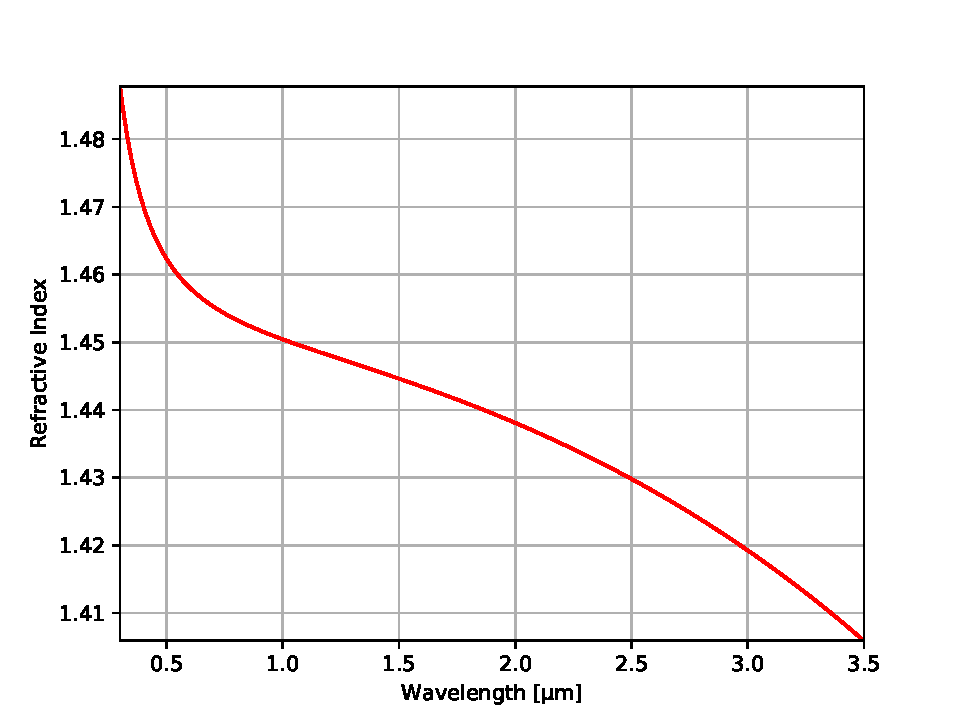
\includegraphics[width = 0.6\textwidth]{Figures/silica_refractive_index.pdf}
\caption{Plot of the calculated refractive index of silica using the Sellmeier equation above from a wavelength of $0.3\mu m$ to $3.5\mu m$}
\label{fig:ri_silica}
\end{figure}
